%!TEX root = ClementiBarba2020.tex

\subsection{Replication of results from Rockstuhl, et al., 2005}

%%% Rockstuhl work summary%%%%
The work of Rockstuhl et al.\cite{rockstuhl2005} study the phonon-polariton response of silicon carbide (SiC)
nanoparticles using the boundary element method. They analyze different "cylindrical particles"
made of 6H-SiC as a function of geometrical cross section. These "cylinders" have an infinite
extension in the third dimension, and they solve these geometries numerically with a 2D 
boundary element method from their previous work \cite{rockstuhl2003}. 
%%% Rockstuhl work summary%%%%

We decided to replicate one of the results that they present on Fig.14 of their paper, which 
presents the scattering cross section of a SiC rectangular cylinder for three different object 
sizes. To comply with our quasistatic approach ($\lambda > d$ where $d$) we chose the particular 
case where a=672 nm and b=328 nm.

\textbf{Difference between methods, mesh and dielectric data}

\textit{method}: The main difference between Rockstuhl simulations and ours is that they solve a 2D problem, 
while we solve a 3D model. In our case the geometry has a finite third dimension. To cope with this
we will extend the third direction considerably, and study this effect.
We compute extinction cross section (scattering plus absorption) while Rockstuhl work present only scattering. 
But since in both scattering and absorption the resonance occur at the same wavelengths, the results are 
comparable.

\textit{mesh}: Their work does not provide any details regarding the discretization of their geometries or 
parameters involved in the simulations. We performed a grid independence study to make sure that we are
solving properly the physics and minimizing errors due to discretization. 

\textit{dielectric data}: The use 6H-SiC as material, and they obtained their data from a a source that we
were not able to replicate. Instead we are using experimental data for 4h-SiC that was provided to us 
via private communications.  

\subsubsection{Grid independance study}

We performed a grid independence study on a SiC cube of side $L=535$ nm submerged in air, under a 
constant electric field aligned with the z-axis.
(similar to quadratic cylinder on Fig 18 of Rockstuhl et.al). 
Due to the nature of the geometry, and its sharp edges it was challenging to see proper convergence. However,
for this type of physics, convergence has been studied in our previous work \cite{ClementiETal2019}. 
In the Figure \ref{fig:cube535} we show a grid independence study, where we go from a mesh of 15552 
triangles (density = 1.11x10$^-4$ $N/\text{\AA}$) to 19200 (density = 9.05x10$^-5$ $N/\text{\AA}$) 
triangles and the computed results do not change.

\begin{figure}
    \centering
    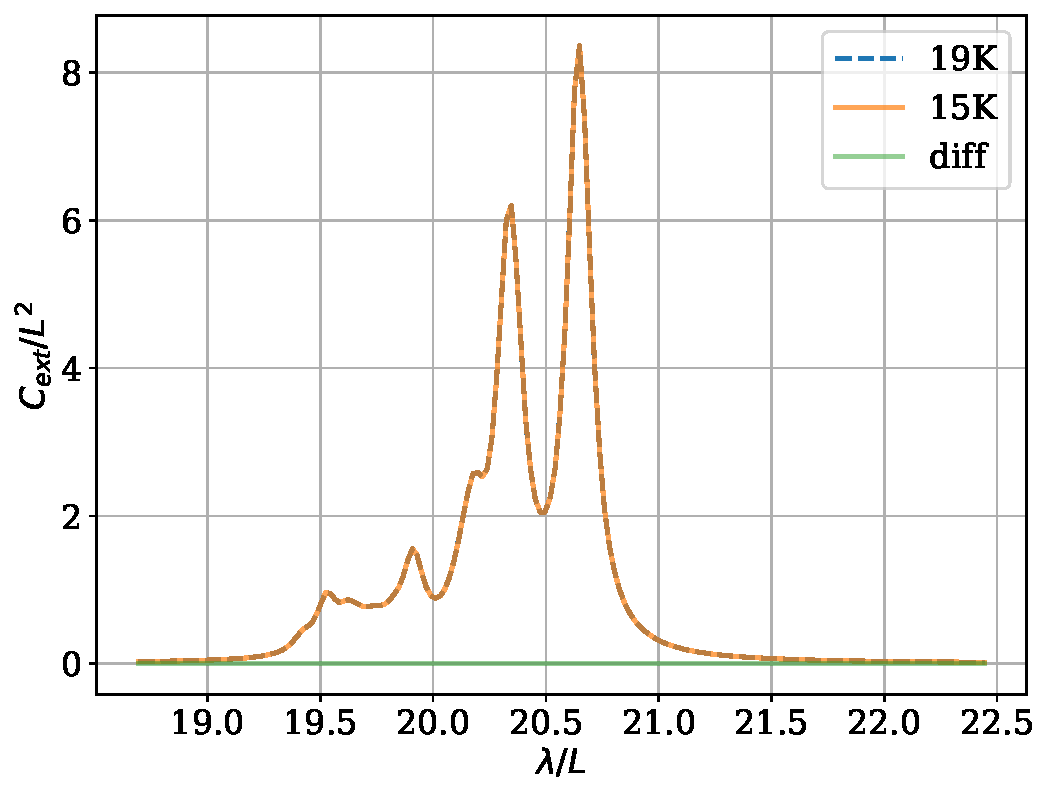
\includegraphics[width=0.85\textwidth]{cubeL535nm_15Kvs19K.pdf} 
    \caption{Grid independence study for a SiC cube of side $L=535 nm$ submerged in air under a constant 
    electric field in the z-direction. The curves represent the extinction cross section divided by $L^2$ 
    as a function of wavelength divided by $L$}
    \label{fig:cube535}
 \end{figure}

It is worth noting that the extinction cross section curve in Figure \ref{fig:cube535} has extra peaks, 
compared to the results of Figure 18 on Rockstuhl, this is due to the 3D nature of our case and the sharp 
edges. This will be approach in the following results where we attempt a replication of one of teh results 
of Figure 14 of Rockstuhl work.

\subsubsection{Replication of Figure 14 (case a1) of Rockstuhl 2005}

We chose to replicate the result of Rocksuthl et al. presented in Figure 14. In particular the case where $a=672$ nm 
and $b=328$ nmn, since these dimension comply with the requirements of the quasistatic approximation.
They present the normalized scattering cross section of a SiC rectangular cylinder, and they perform simulation 
for two different setups. In Rockstuhl Figure 14 (left) they have the wave vector (illumination) along the long 
side of the geometry, which means that the electric field is parallel to the short side of the rectangle. Following, 
a similar analysis Rockstuhl Figure 14 (right) they have the wave vector (illumination) along the short
side of the geometry, which means that the electric field is parallel to the long side of the rectangle. These orientations,
correspond to the images (A) and (B) in the sketch presented in Figure \ref{fig:rectangle_sketch}.

Based on the results of the grid independence stud we decided to we used the density of the cube as a reference to 
produce the meshes for the replication of figures 14a and 14b on Rockstuhl's work (case a1=672, b=328). For the third 
dimension we needed to chose a value that represents "infinity". To achieve this, we perform a study on the effects of 
elongate the third dimension. In Figure \ref{fig:ext_y_14} we present the results for two different values of the 
third dimension, $y=1344$ nm (2xa) and $y=2688$ nm (4xa). 
We see that as we extend the third dimension the intensity of some peaks decreases, this is because some
of the peaks are related to the third dimension. Therefore, from now on we use $y=y=2688$ nm. It is worth 
noting that we could have increased this value more, however, the simulations will become computational
more expensive and we will still have the effects of having a 3D model.

\begin{figure}
    \centering
    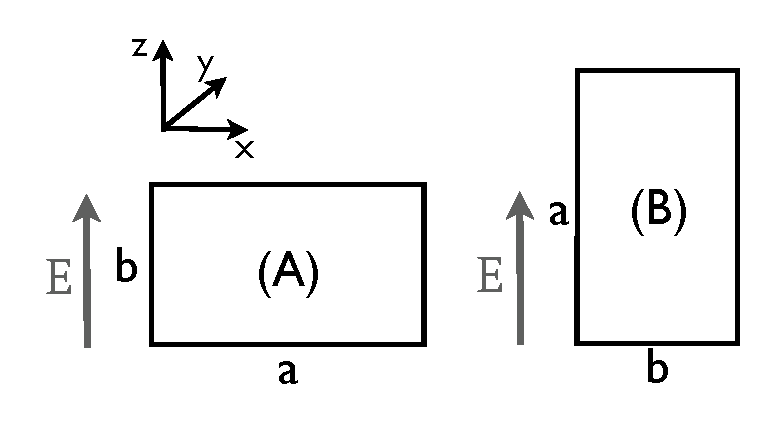
\includegraphics[width=0.45\textwidth]{rockstuhl_rectangles.pdf} 
    \caption{Rockstuhl runs configurations}
    \label{fig:rectangle_sketch}
\end{figure}

\begin{figure}
    \centering
    \subfloat{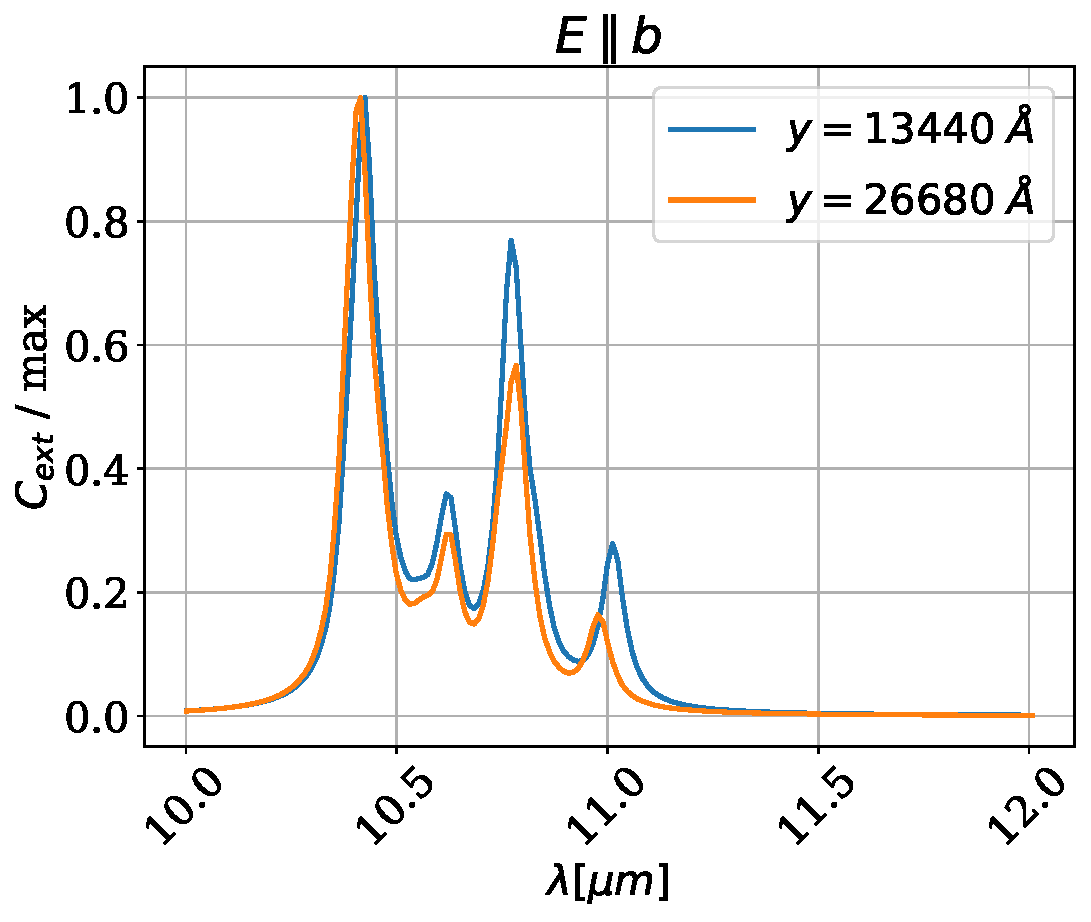
\includegraphics[width=0.45\textwidth]{ext_y_14a.pdf}}
    \subfloat{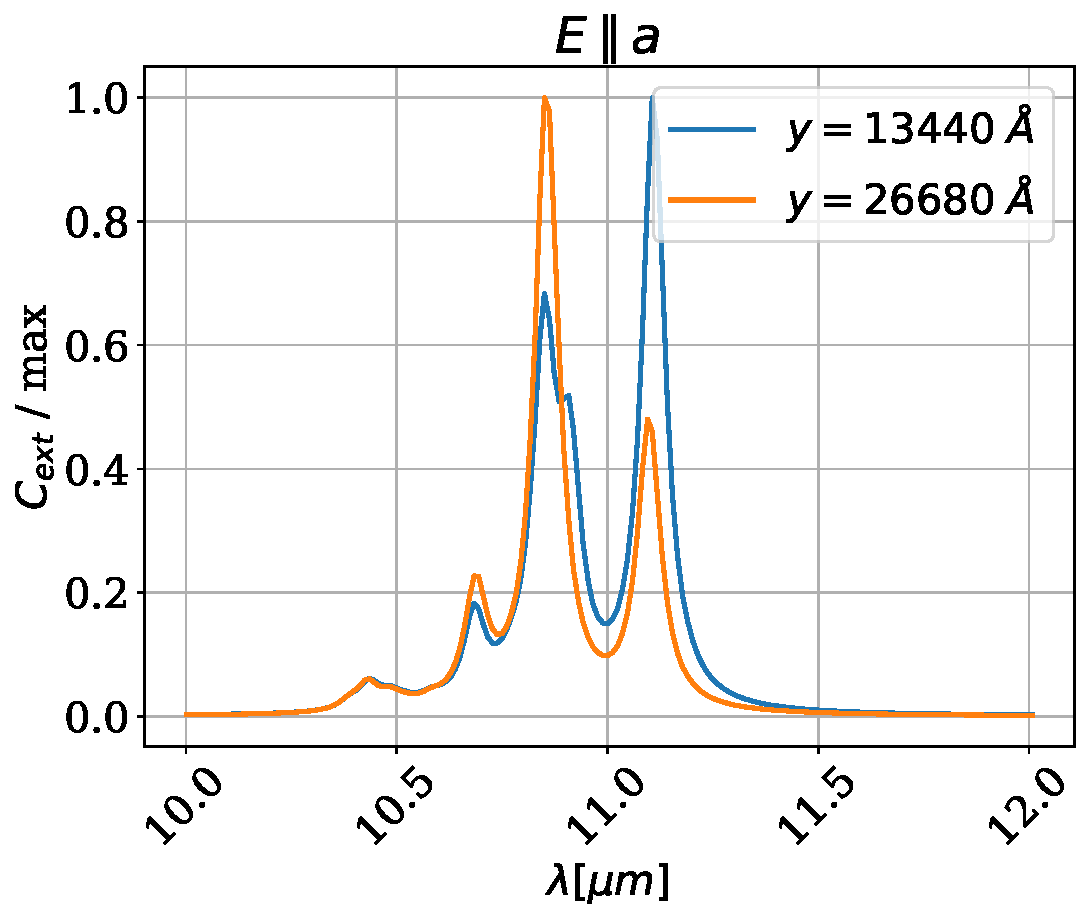
\includegraphics[width=0.45\textwidth]{ext_y_14b.pdf}} 
    \caption{Effect of the elongation of the third direction ($y$) on the 
        extinction cross section of a rectangular prism of SiC of dimensions $a=672$ nm 
        and $b=328$ nm, submerged in air and under a constant electric field 
        parallel to the z-axis. The left plot corresponds to a configuration such that the electric 
        field is parallel to $b$ (configuration (A) on Figure \ref{fig:rectangle_sketch}), while the 
        right plot corresponds to a configuration such that the electric field is 
        parallel to $a$ (configuration (B) on Figure \ref{fig:rectangle_sketch}}
    \label{fig:ext_y_14}   
 \end{figure}


To generate the meshes for these simulations, we used the open source software Trimesh 
(\url{https://github.com/mikedh/trimesh}), but we realized that it was not producing a 
uniform mesh and that it was not possible to produce regular triangles with the functions 
available. To overcome this, we created our own mesh using python scripts, and therefore 
obtain uniform meshes. We wanted to study the effect of a uniform mesh as well as the effect
on rounding the edges. We wanted to round the edges since in Rockstuhl work this was mentioned 
as a factor that will introduce extra peaks on the response. We were not able to control the 
roundness as a function of arc of curvature or the dimensions of the rectangular prism, so we 
decided to use the default settings on Trimesh. Figure \ref{fig:tri_reg_round_14} shows the 
results on the effect of uniformity and roundness. You can see that the second peak is not
present in the green curve, which can be attributed to the effect of the roundness. This is 
consistent with the results on Rockstuhl's work. 

\begin{figure}
    \centering
    \subfloat{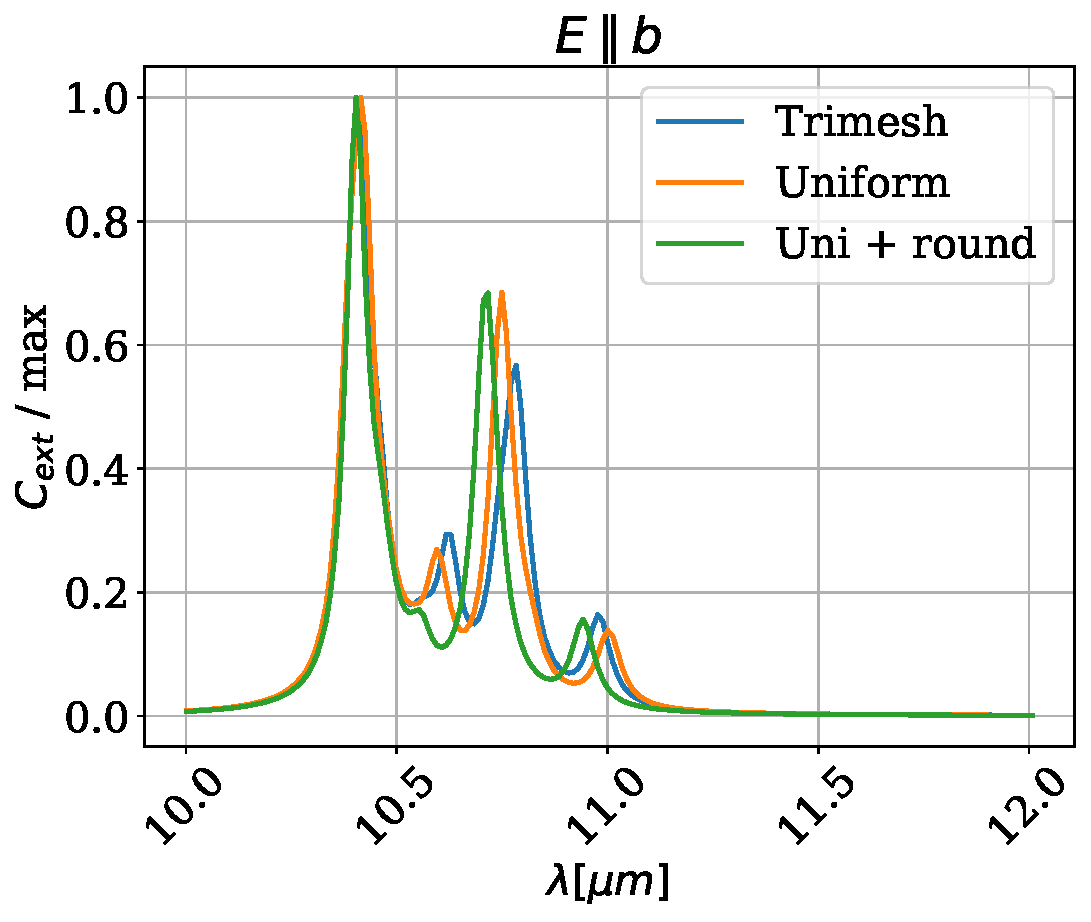
\includegraphics[width=0.45\textwidth]{tri_reg_round_14a.pdf}}
    \subfloat{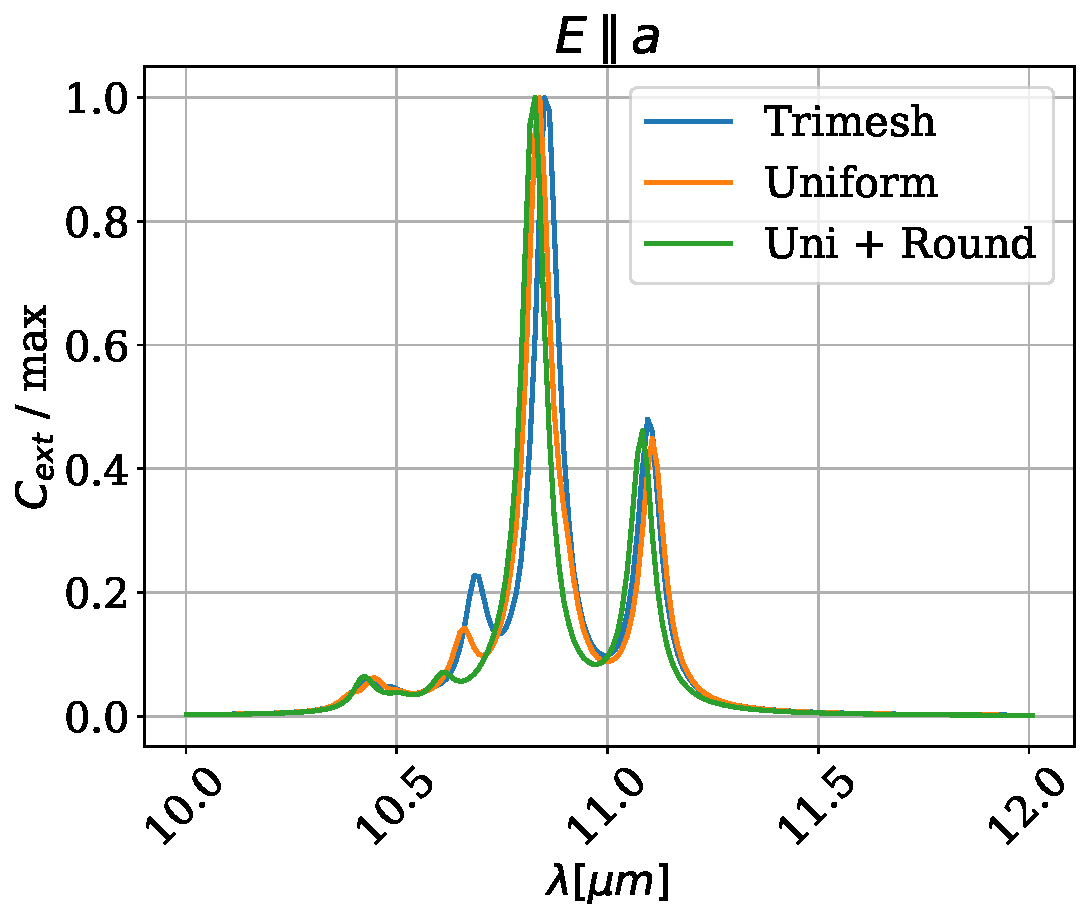
\includegraphics[width=0.45\textwidth]{tri_reg_round_14b.pdf}}
    \caption{ Effect of uniformity and roundness on the mesh on the 
    extinction cross section of a rectangular prism of SiC of dimensions $a=672$ nm, 
    $b=328$ nm and $y=2688$ nm, submerged in air and under a constant electric field 
    parallel to the z-axis}
    \label{fig:tri_reg_round_14}
 \end{figure}

Once we have found the "best" possible geometry approximation, we show how our results 
(green curve in Figure \ref{fig:tri_reg_round_14}) compare 
with the original results from Rockstuhl's Figure 14. We have obtained Rockstuhl's curves by using 
the WebPlotDigitizer (\url{https://apps.automeris.io/wpd/}). The replication results are 
presented in Figure \ref{fig:rep_14}. We can say that the main peaks presented in Rockstuhl et al. are 
successfully replicated. While we still have the presence of a third peak in our results, we believe 
this is a consequence of the 3D nature of our geometry.

 \begin{figure}
    \centering
    \subfloat{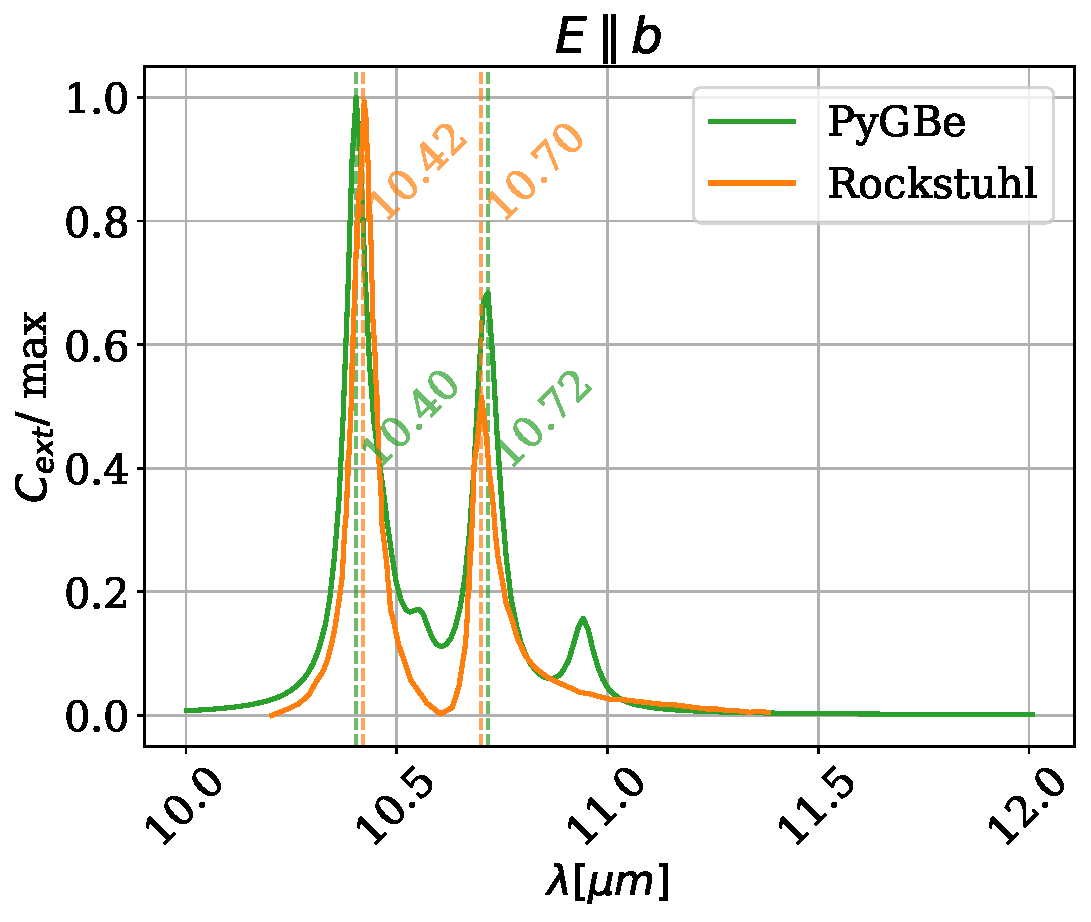
\includegraphics[width=0.45\textwidth]{replication_14a.pdf}}
    \subfloat{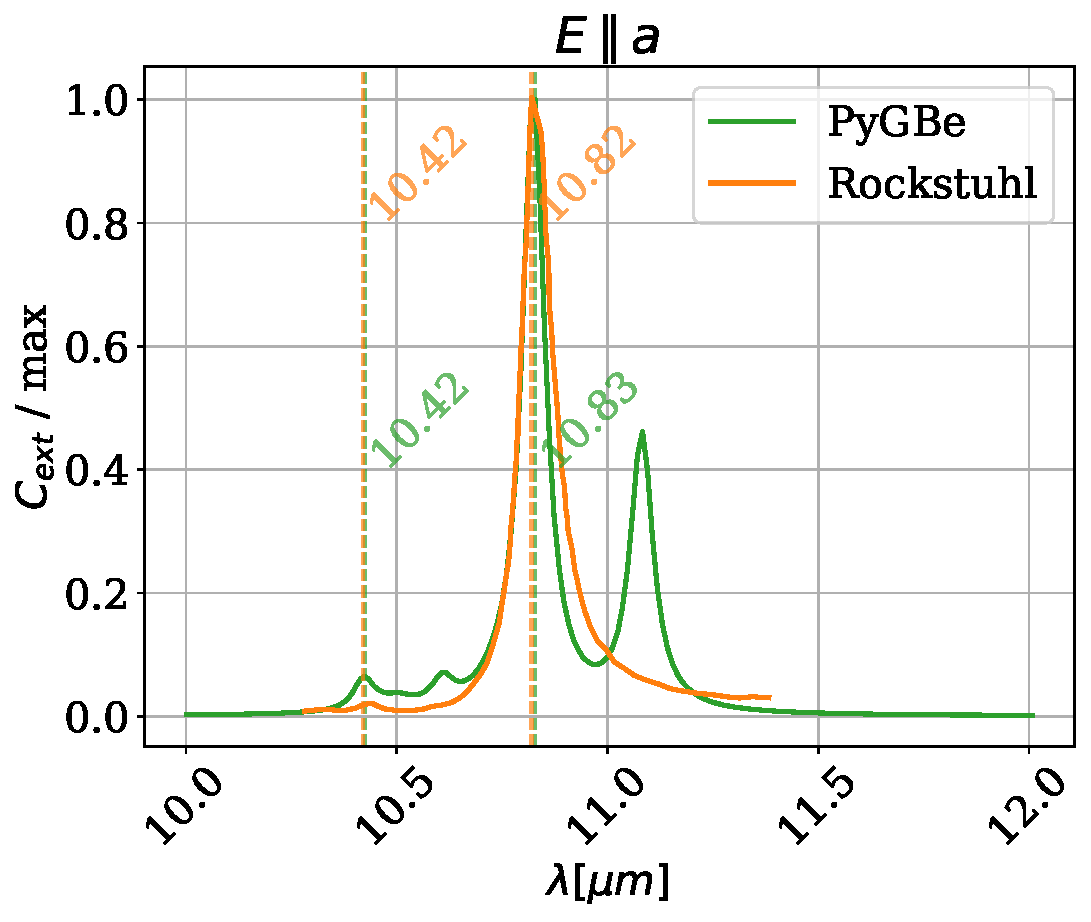
\includegraphics[width=0.45\textwidth]{replication_14b.pdf}} 
    \caption{Replication of Figure 14 from Rockstuhl 2005. Extinction cross section of a
    rectangular prism of SiC of dimensions $a=672$ nm, $b=328$ nm and $y=2688$ nm, submerged
    in air and under a constant electric field parallel to the z-axis.}
    \label{fig:rep_14}
 \end{figure}


 \subsection{Replication of results from Ellis et al., 2016, and validation}

 %%% Ellis work summary %%%%
The work of Ellis and coworkers \cite{ellis2016} study the aspect-ratio evolution of high-order
resonant modes in localized surface phonon-polariton nanostructures. They study the
excitation of multipolar localized surface phonon polaritons (SPhP) resonances, by measuring
polarized reflectance measurements on 4H-SiC pillars of fixed height ($H=950$ nm), fixed 
width ($W=400$ nm) and varied length ($L=400-4800$ nm) and therefore an aspect ratio
($AR=L/W=1-12$). These pillars are patterned on a squared grid with a pitch $P=L+500$ nm
to reduce coupling. In their simulations and experiments they excite the localized SPhP
resonances, they perform polarized reflectance measurements with the incident polarization 
oriented parallel or perpendicular to the long axis of the pillars.  
 %%% Ellis work summary %%%%

We aim to replicate the computational result presented in Figure S4 of their supplementary 
material (NOT SURE HOW TO CITE THIS) that correspond to the black curve on their plot. In this 
figure they show simulation results for the resonance spectral position of the lower frequency 
mode when having parallel polarization ($E^{\parallel}_{100}$), with an incidence angle of 22$^\circ$.
We first attempted to replicate this result since they have simulations with the gap between pillars 
is 5000 nm, and this cause negligible coupling. This result is suitable to compare with 
what we can model using \pygbe.  




\textbf{Difference between methods, mesh and dielectric data}

\textit{methods}
In Ellis et al simulations they solve full Maxwell equations via the RF package of the finite
element method software COMSOL. To represent the array of pillars and their interactions, they use
periodic boundary conditions of one pillar over a portion of substrate. They present the reflectance 
as a function of the wave number. As we mentioned before, we use the boundary element method in 
the quasistatic approximation, which is suitable in these case since Ellis pillar's size is small 
compared to the wavelength involved in the simulations (800-1000 cm$^-1$). We measure extinction cross 
section, which will express as peaks instead of inverted peaks (as in reflection) since you see maximum
extinction when there is minimum reflection. The intensity of the peaks is not comparable, but we are 
looking to match the wave number at which these events happen. 

\textit{mesh}
For the case of aspect ratio AR=4 we count with a triangular surface mesh provided by the authors of 
Ellis et al. Which is a non-structured mesh of approximately 4 thousand elements. To produce the remaining 
meshes, we use our python script to generate a uniform mesh and round the edges using Trimesh. 
After doing certain refinement studies we noticed that to achieve close results to the original mesh, using a
uniform mesh, we needed to double the density (I HAVE SOME PLOTS ON THIS RESULTS BUT 
I'M NOT SURE IF WE WANT TO PUT THEM, SINCE WE DON'T HAVE SPACE).
To replicate the results of figure S4 on their supplementary material, we use uniform meshes. While for the 
replication of figure 2a and the validation result we used the mesh provided by the authors of Ellis et al. 


\textit{dielectric data}
The dielectric data for the simulations, was given by the authors of the paper via a private communication. 

To be able to replicate this results, we need to identify the lower frequency mode for each of
the aspect ratios in our computations. For each aspect ratio (AR) 
value from 1 to 7 we computed the extinction cross section $C_{ext}$ across the wave number in the range
800-1000 $cm^{-1}$. We identify the lower frequency mode ($E^{\parallel}_{100}$ in Ellis paper)  that is not a 
longitudinal mode (mode related to the hight of the pillar, only visible when the incidence of the 
electric field is not normal). We can identify the longitudinal modes by comparing normal vs 22 degrees 
angle of incidence runs. As we mentioned the longitudinal modes, due to its nature, do not appear when we 
have the normal incidence . Then, on the 22 degree incidence computations we choose the lower wave number mode
that it's not a longitudinal mode. 

Figure \ref{fig:AR_22_vs_norm} show the results of the extinction cross section of a SiC pillar of fixed
height ($H=950$ nm), fixed width ($W=400$) and varied length ($L=400-2800$ nm). The simulations where performed 
performed for the Long Edge orientation, meaning that the electric field is aligned with the length pillar 
when having normal incidence. (I SHOULD PROBABLY MAKE A DIAGRAM OF THIS)

In Figure \ref{fig:AR_22_vs_norm} and Table \ref{tab:ar_peaks} we show the resonance peaks and
their corresponding wavelengths. In the table we mark in bold the peaks which correspond to 
the $E^{\parallel}_{100}$ mode. 

\begin{figure}
    \centering
    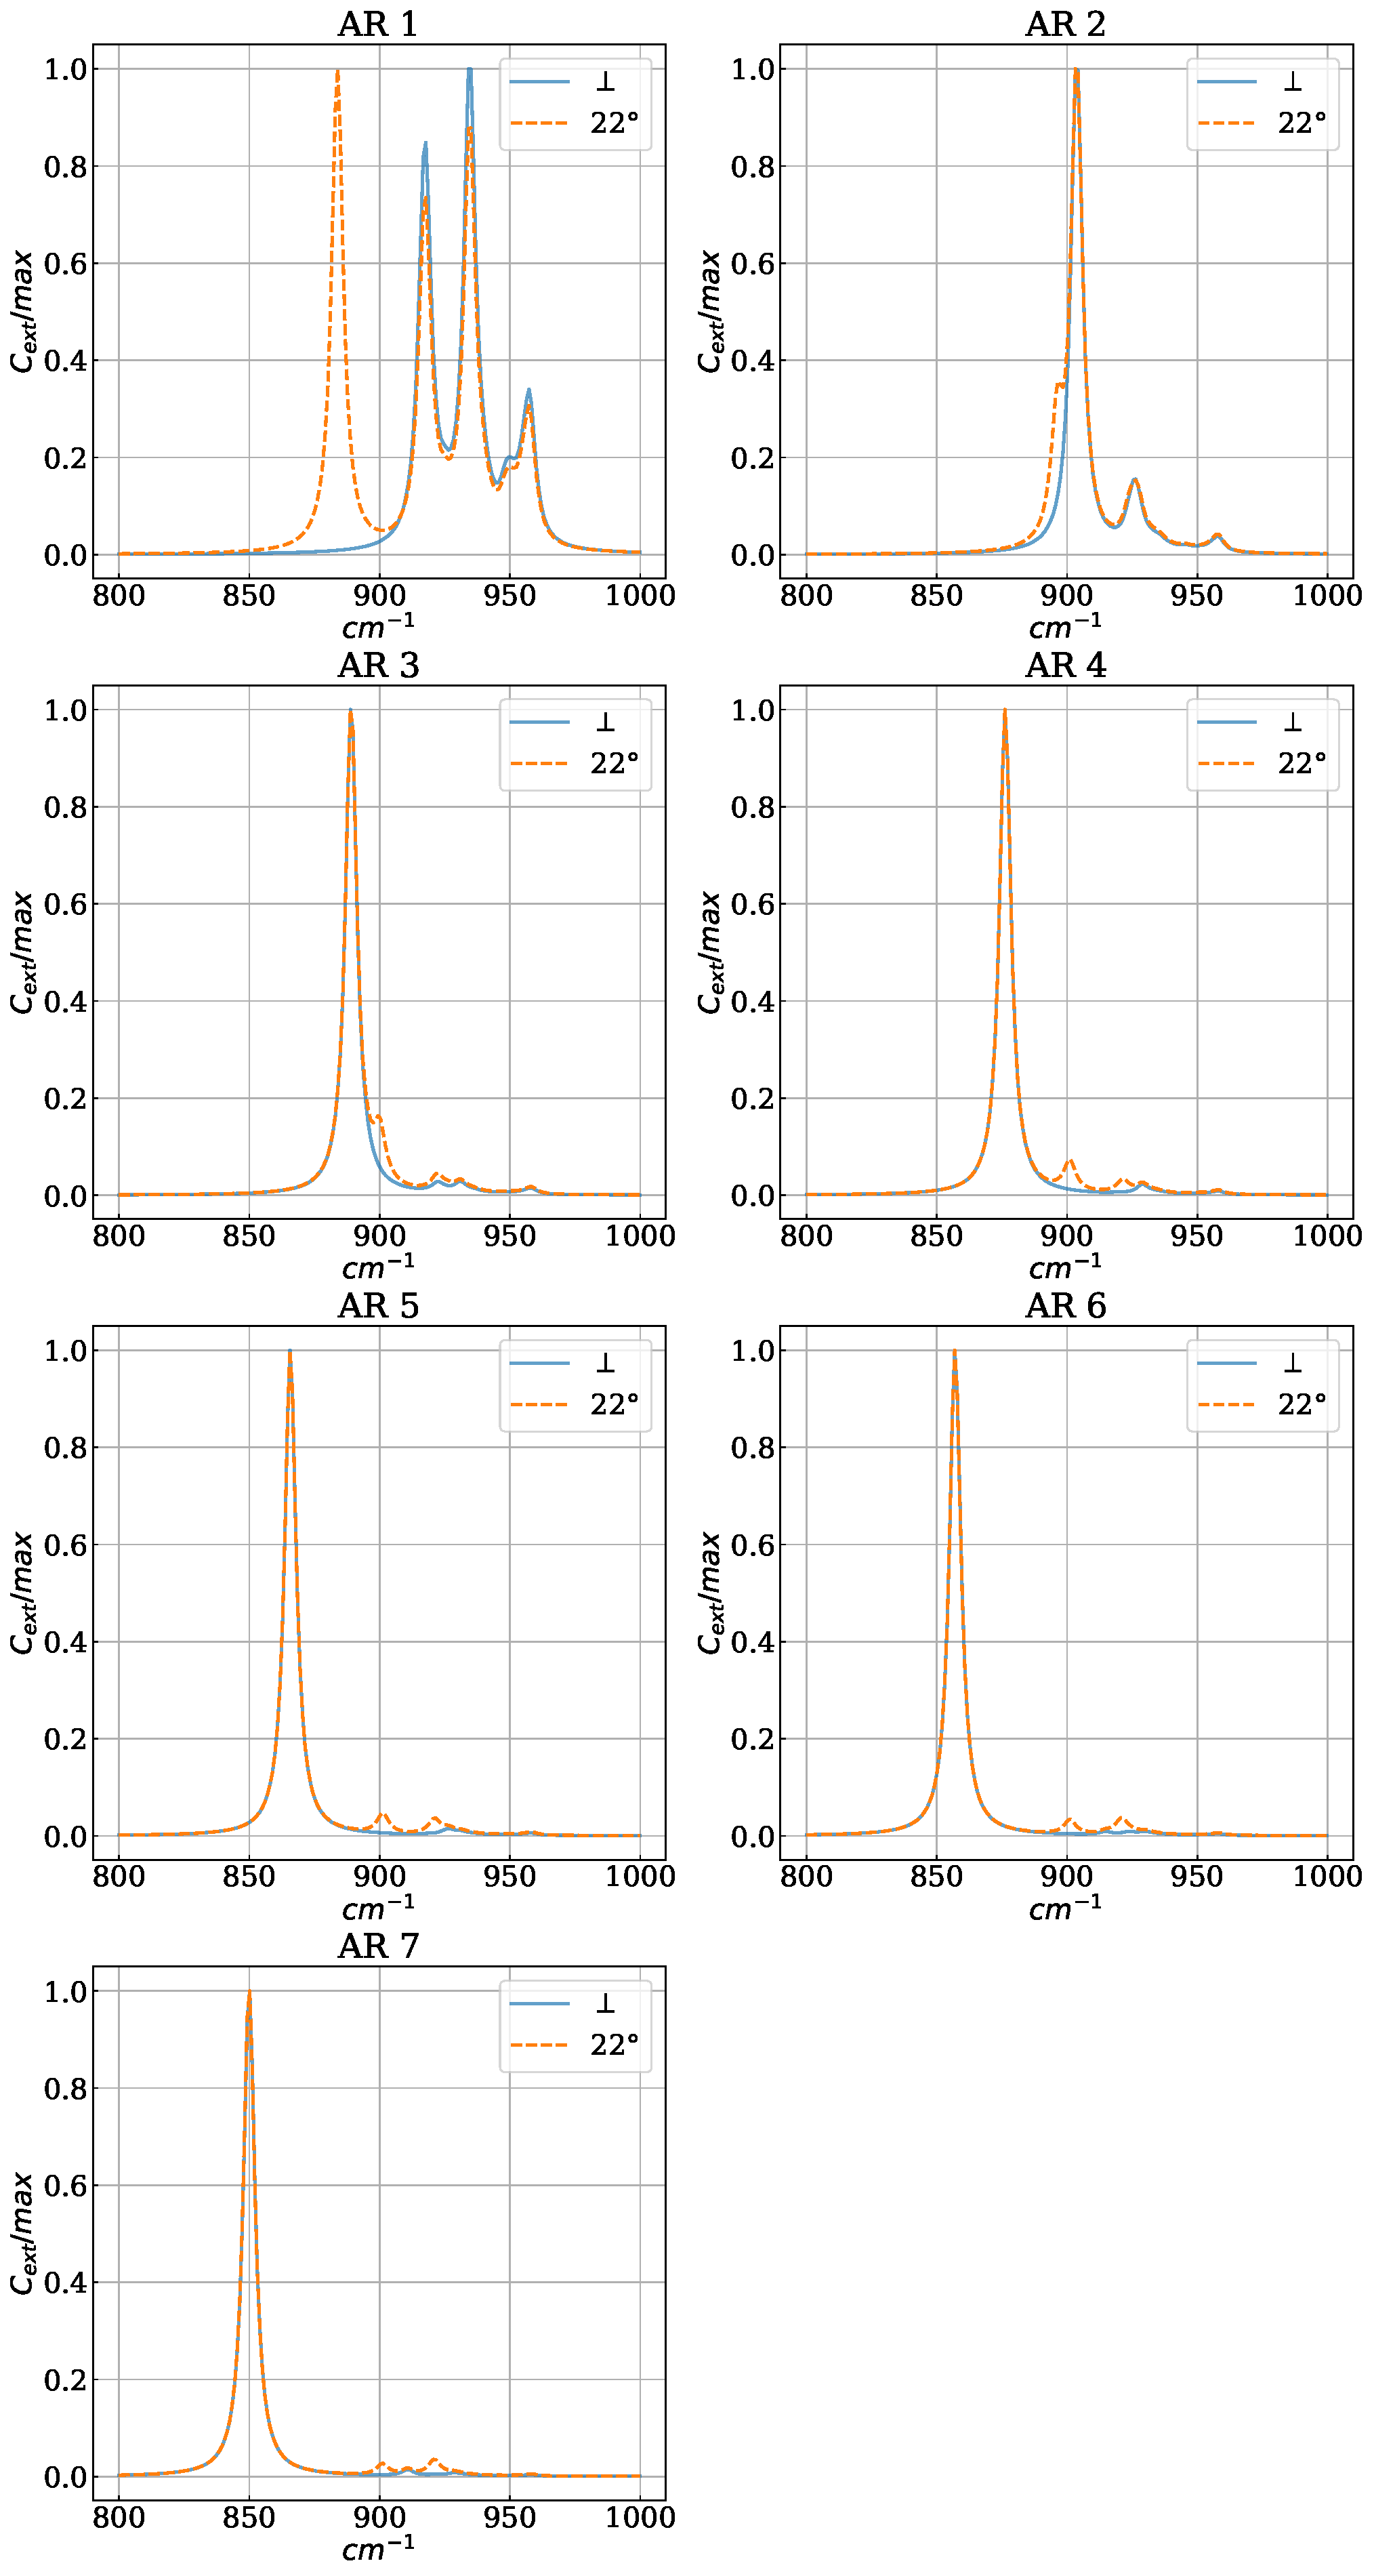
\includegraphics[width=0.85\textwidth]{AR_22_vs_norm.pdf} 
    \caption{Extinction cross section across wave number for SiC pillars of multiple aspect ratios,  
             (H=950 nm, W=400nm, L=400-2800 nm (AR=1-7)), where we have normal incidence and a 
             22 degrees incidence.
            }
    \label{fig:AR_22_vs_norm}
 \end{figure}


\begin{table}
    \begin{center}
      \caption{Wavelength at which peaks happen for different aspect ratios, for runs where the electric
      field is parallel to the length (L) of the pillar. We have normal incidence and 22 degrees.}
      \label{tab:ar_peaks}
      \begin{tabular}{c c c c c c c c}
        \textbf{AR} \\
        \hline
        \multirow{2}{*}{1} & $\perp$ & \textbf{917.73} & 934.092 & 949.604 & 957.325 \\ % <-- Combining 2 rows with arbitrary with (*) and content 12
        & 22$^{\circ}$ & 883.926 & \textbf{917.73} & 935.052 & 949.604 & 957.325 \\ % <-- Content of first column omitted.
        \hline
        \multirow{2}{*}{2} & $\perp$ & \textbf{903.233} & 926.395 & 944.762 & 958.242 \\ % <-- Combining 2 rows with arbitrary with (*) and content 12
        & 22$^{\circ}$ & 896.517 & \textbf{903.233} & 926.395 & 944.762 & 958.242 \\ % <-- Content of first column omitted.
        \hline
        \multirow{2}{*}{3} & $\perp$ & \textbf{888.793} & 922.552 & 931.223 & 948.613 & 958.242 \\ % <-- Combining 2 rows with arbitrary with (*) and content 12
        & 22$^{\circ}$ & \textbf{888.793} & 899.418 & 922.552 & 931.223 & 958.242 \\ % <-- Content of first column omitted.
        \hline
        \multirow{2}{*}{4} & $\perp$ & \textbf{876.186} & 929.32 & 946.639 & 958.242 \\ % <-- Combining 2 rows with arbitrary with (*) and content 12
        & 22$^{\circ}$ & \textbf{876.186} & 901.281 & 921.618 & 929.32 & 945.745 & 958.242 \\ % <-- Content of first column omitted.
        \hline
        \multirow{2}{*}{5} & $\perp$ & \textbf{865.576} & 926.395 & 945.745 & 958.242 \\ % <-- Combining 2 rows with arbitrary with (*) and content 12
        & 22$^{\circ}$ & \textbf{865.576} & 901.281 & 921.618 & 958.242 \\ % <-- Content of first column omitted.
        \hline
        \multirow{2}{*}{6} & $\perp$ &  \textbf{856.904} & 914.793 & 923.489 & 929.32 & 946.639 & 958.242\\ % <-- Combining 2 rows with arbitrary with (*) and content 12
        & 22$^{\circ}$ & \textbf{856.904} & 901.281 & 920.6 & 958.242\\ % <-- Content of first column omitted.
        \hline
        \multirow{2}{*}{7} & $\perp$ &  \textbf{850.134} & 910.963 & 921.618 & 928.372 & 946.639 & 958.242 \\ % <-- Combining 2 rows with arbitrary with (*) and content 12
        & 22$^{\circ}$ & \textbf{850.134} & 901.281 & 910.963 & 920.6 & 958.242\\ % <-- Content of first column omitted.
        \hline
      \end{tabular}
    \end{center}
  \end{table}

Once we identify the proper modes, we proceed to the replication of Figure S4 on the 
supplementary material of Ellis et al work. It is worth mentioning that we limit ourselves to
the replication of the black curve in their plot, since in this case the pillars are separated 
by 5000 nm which means the coupling effects are negligible. Figure \ref{fig:rep_FS4_ellis} shows
the results from  Ellis et al (digitized using the WebPlotDigitizer) and the results obtained
with \pygbe, and Table \ref{tab:err_AR} shows that the percentage error is below 2$\%$ for all
the cases


\begin{figure}
    \centering
    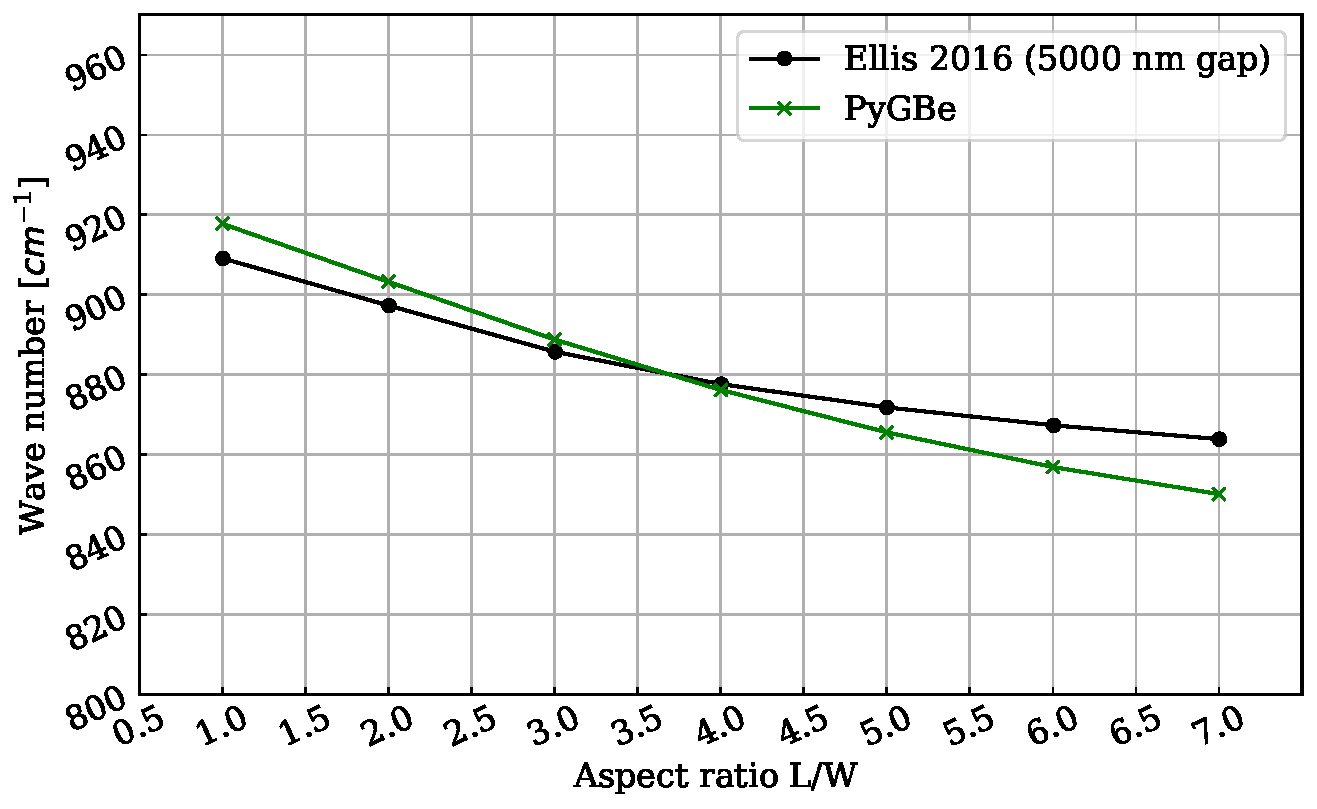
\includegraphics[width=0.85\textwidth]{AR_rep_FS4_Ellis2016.pdf} 
    \caption{Replication of figure S4 of supplementary material of Ellis 2016. Wave
    number at which happens the $E^{\parallel}_{100}$ mode for different aspect ratios.}
    \label{fig:rep_FS4_ellis}
 \end{figure}
 
 \begin{table}
    \centering
    \caption{Percentage error for different aspect ratios.} 
    \label{tab:err_AR}
    \begin{tabular}{c c}
    \hline%\toprule
    AR & \% error \\
    \hline%\midrule
     $1$ & $0.95$ \\
     $2$ & $0.67$ \\
     $3$ & $0.35$ \\
     $4$ & $0.16$ \\
     $5$ & $0.72$ \\
     $6$ & $1.20$ \\
     $7$ & $1.59$ \\
    \hline%\bottomrule
    \end{tabular}
\end{table}

\subsubsection{Validation of \pygbe against Fig 2a experimental results}

For the case of aspect ratio four (AR=4) we obtain the smallest error using the uniform
mesh. Since we count with the mesh provided by the authors, and knowing that our computation 
for the mode $E^{\parallel}_{100}$ compares well with their computations, we attempted to 
validate our simulations with their experimental results (red curve on paper), as well 
as to replicate their simulations (green curve on paper) on Figure 2a of their paper.
Figure 2a of Ellis et al, presents measured and simulated reflectance of SiC pillar
arrays with a 500 nm gap. All their measurements and simulations were performed with 
22$^\circ$ off-normal angle of incidence and incoming polarization parallel to the 
elongated size of the pillar. 

Using \pygbe we compute the extinction cross section of an isolated SiC pillar (AR=4)
with no substrate, submerged in air under a constant electric field in the z-direction, 
and rotate the orientation of the pillar to match the angle of incidence. 
(SHOULD PROBABLY PUT A DIAGRAM OF THIS). In Figure \ref{fig:pygbe_vs_exp_2a} we present 
comparison of our simulations and the experimental results from Ellis et al. There is a 
difference in the peaks wavelength that is noticeable. This could be attributed to the
fact that in their experiments the separation between pillars is of 500 nm, which implies
there are coupling effects that in our simulations are not contemplated.  

\begin{figure}
    \centering
    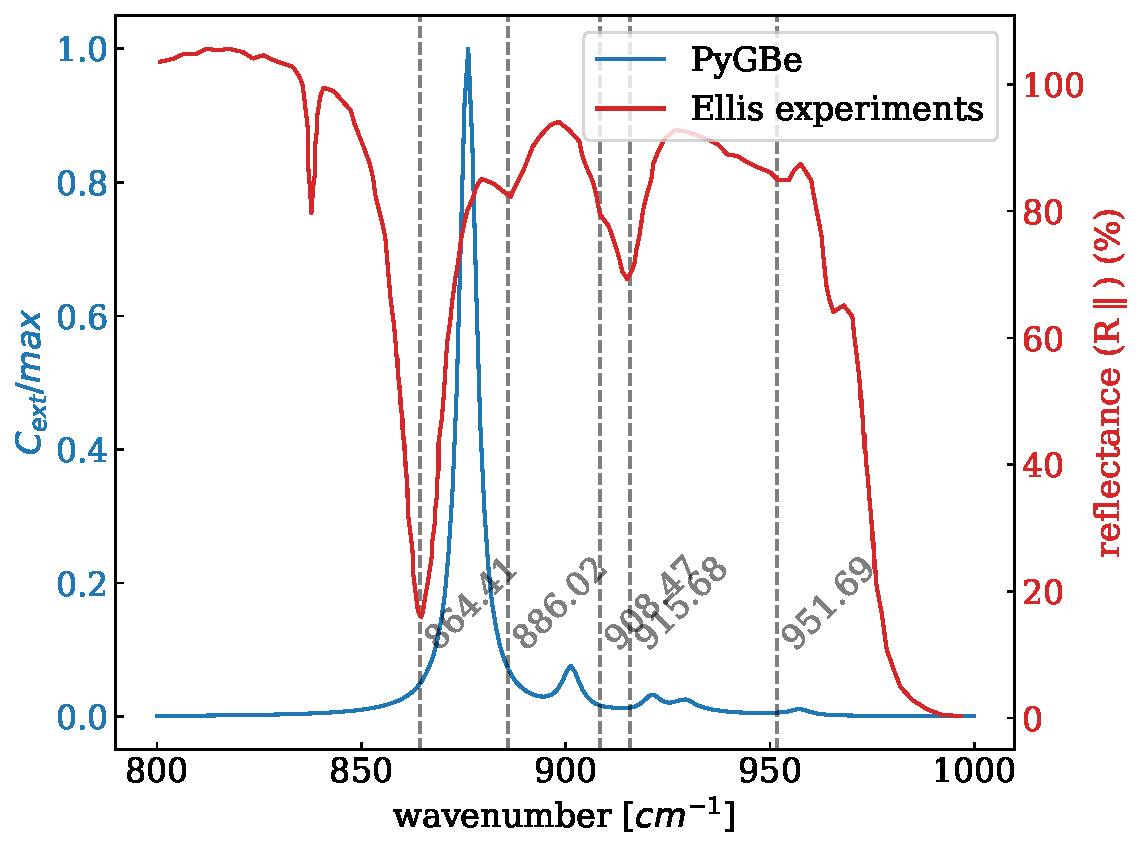
\includegraphics[width=0.85\textwidth]{pygbe_vs_exp_fig2a_Ellis.pdf} 
    \caption{\pygbe vs experiments of figure 2a of Ellis 2016. Ellis data 
    was digitized with web digitizer.}
    \label{fig:pygbe_vs_exp_2a}
 \end{figure}

\paragraph{First order correction}

Since our simulations do not count for coupling effects, we can not strictly imitate 
the conditions to validate our solver. However, from Figure S4 on the supplementary 
material of Ellis et al, we know that coupling effects affect the $E^{\parallel}_{100}$ 
mode by a shift of 12.17 cm$^-1$. Therefore as a \textit{first order correction} we can 
subtract this value from our simulations, to contemplate for coupling effects. In Figure 
\ref{fig:val_2a} we present the result after applying the correction for coupling effects. 

\begin{figure}
    \centering
    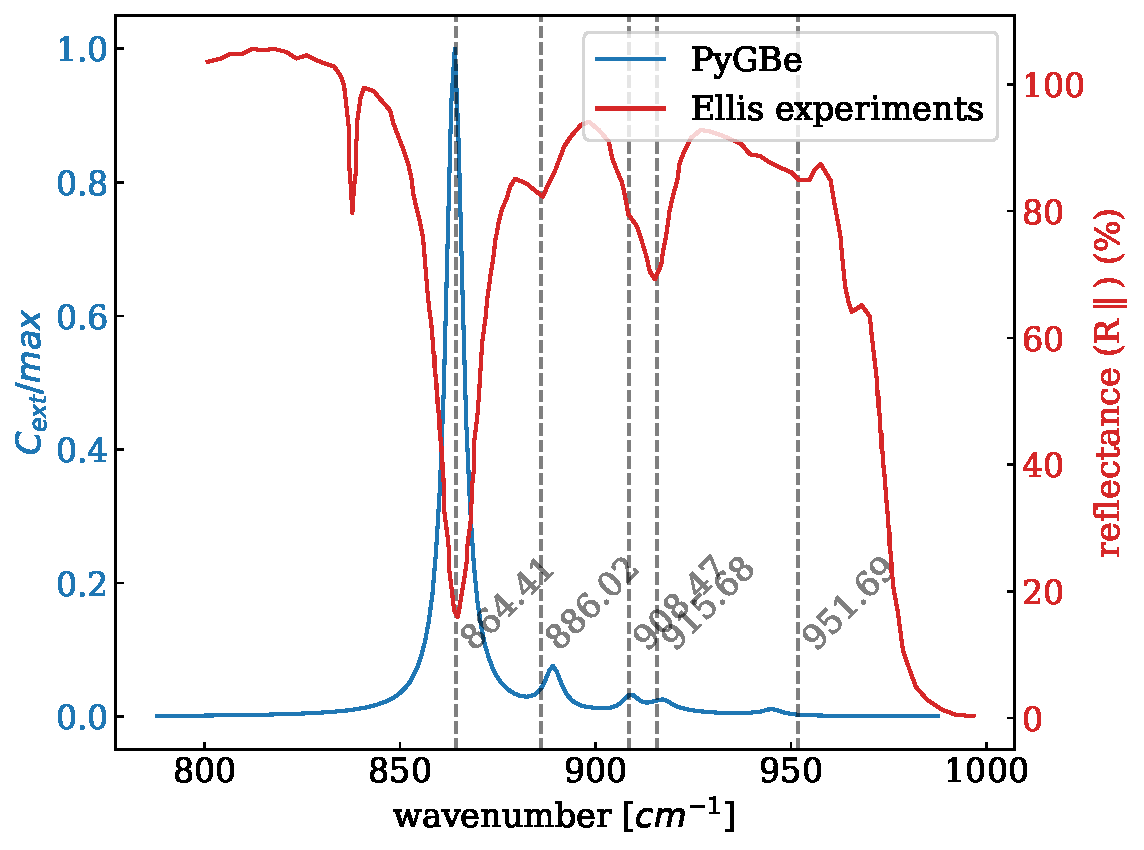
\includegraphics[width=0.85\textwidth]{validation_FOA_fig2a_Ellis.pdf} 
    \caption{Validation against experiments in figure 2a of Ellis 2016, using first order approximation}
    \label{fig:val_2a}
 \end{figure}

If we use the same approximation and compare the results with Ellis simulations on
Figure 2 of their paper (green curve) we get (see Figure \ref{fig:rep_2a})

\begin{figure}
    \centering
    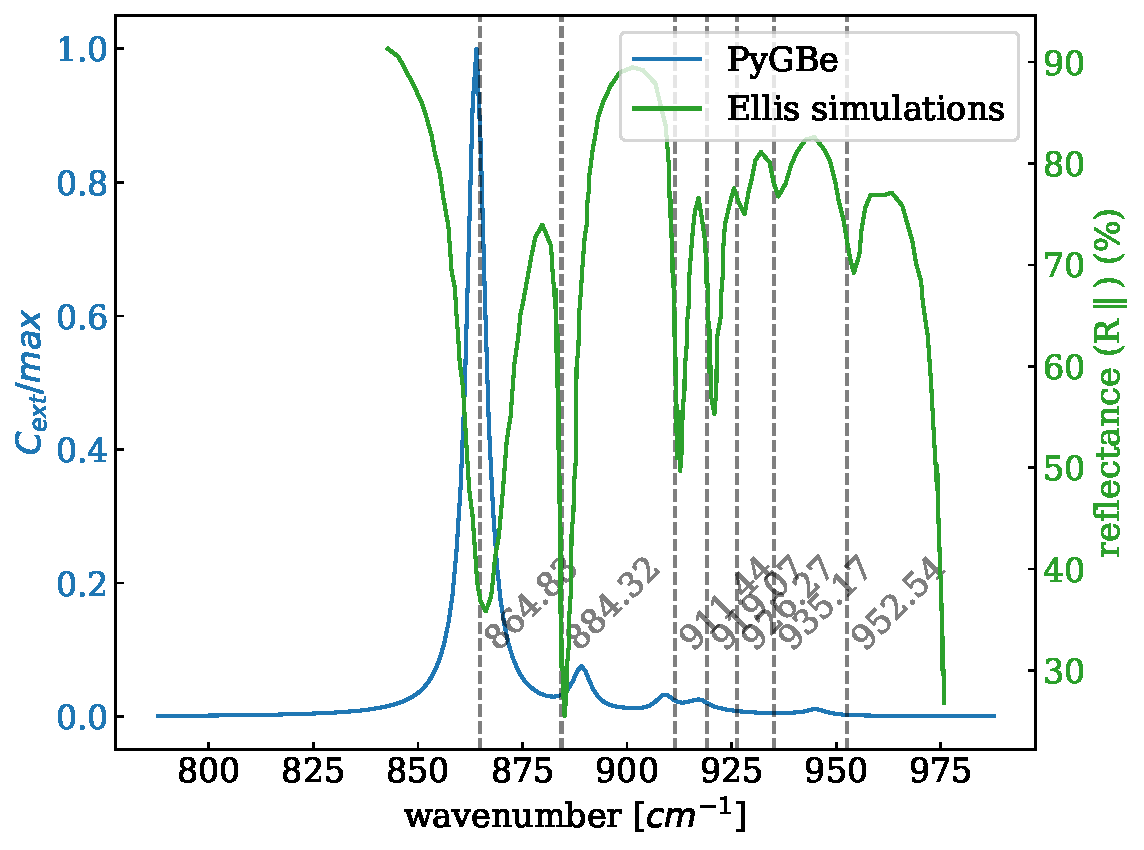
\includegraphics[width=0.85\textwidth]{replication_FOA_fig2a_Ellis.pdf} 
    \caption{Replication of simulations in figure 2a of Ellis 2016, using first
     order approximation}
    \label{fig:rep_2a}
 \end{figure}